\documentclass[a4paper]{article}
\usepackage{import}
\usepackage{graphicx}
\usepackage{float}
\usepackage{pgfplots}
\usepackage{listings}
\usepackage{enumitem}
\usepackage{textcomp}
\usepackage{tikz}
\usetikzlibrary{decorations.pathreplacing} % for angle arc
\usetikzlibrary{angles, quotes, calc, positioning, trees} % for drawing angles
\pgfplotsset{compat=1.18,width=10cm}
\usepackage{tikz-cd}
\usepackage{booktabs}
\usepackage{cancel}
\usepackage{amsmath}
\usepackage{minted}
\usepackage{csquotes}
\usepackage{gensymb}
\usepackage{forest}
\usepackage{amsthm}
\usepackage{amssymb}
\usepackage{fontawesome} 
\usepackage{varwidth}
\usepackage{pgfplots}
\usepackage{lipsum}
\usepackage{mdframed} 
\usepackage{color}   
\usepackage{hyperref}
\newmdtheoremenv{theo}{Theorem}
\usepackage{mathtools}
\DeclarePairedDelimiter\ceil{\lceil}{\rceil}
\DeclarePairedDelimiter\floor{\lfloor}{\rfloor}

\hypersetup{
    colorlinks=true, %set true if you want colored links
    linktoc=all,     %set to all if you want both sections and subsections linked
    linkcolor=black,  %choose some color if you want links to stand out
}

% Define theorem styles
\newtheorem{theorem}{Theorem}[section]    % Theorems numbered within sections
\newtheorem{lemma}[theorem]{Lemma}        % Lemmas use the same counter as theorems
\newtheorem{corollary}[theorem]{Corollary} % Corollaries use the same counter as theorems
\newtheorem{proposition}[theorem]{Proposition} % Proposition uses the same counter
\newtheorem{property}[theorem]{Property}
\theoremstyle{definition}
\newtheorem{definition}[theorem]{Definition} % Now uses the same counter as theorems


% Remark-style theorem
\theoremstyle{remark}
\newtheorem{remark}[theorem]{Remark}

% Boxed environment for theorems
\newmdenv[
  linewidth=0.8pt,
  roundcorner=5pt,
  linecolor=black,
  backgroundcolor=white!5,
  skipabove=\baselineskip,
  skipbelow=\baselineskip,
  innerleftmargin=10pt,
  innerrightmargin=10pt,
  innertopmargin=5pt,
  innerbottommargin=5pt
]{thmbox}

% Custom proof environment (also boxed)
\renewenvironment{proof}[1][Proof]{%
  \begin{mdframed}[linewidth=0.8pt, roundcorner=5pt, linecolor=black, skipabove=\baselineskip, skipbelow=\baselineskip, innertopmargin=5pt, innerbottommargin=5pt]%
  \noindent\textbf{#1. }%
}{%
  \end{mdframed}%
}

% Redefine theorem environments to use thmbox
\let\oldtheorem\theorem
\renewenvironment{theorem}{\begin{thmbox}\begin{oldtheorem}}{\end{oldtheorem}\end{thmbox}}

\let\oldlemma\lemma
\renewenvironment{lemma}{\begin{thmbox}\begin{oldlemma}}{\end{oldlemma}\end{thmbox}}

\let\oldcorollary\corollary
\renewenvironment{corollary}{\begin{thmbox}\begin{oldcorollary}}{\end{oldcorollary}\end{thmbox}}

\let\oldproposition\proposition
\renewenvironment{proposition}{\begin{thmbox}\begin{oldproposition}}{\end{oldproposition}\end{thmbox}}

\let\oldproperty\property
  \renewenvironment{property}{\begin{oldproperty}}{\end{oldproperty}}


% Reference shortcuts
\newcommand{\thmref}[1]{Theorem~\ref{#1}}
\newcommand{\lemref}[1]{Lemma~\ref{#1}}
\newcommand{\corref}[1]{Corollary~\ref{#1}}
\newcommand{\propref}[1]{Property~\ref{#1}} 

% To customize QED symbol
\renewcommand{\qedsymbol}{$\blacksquare$}

\usetikzlibrary{decorations.pathreplacing} % for angle arc
\usetikzlibrary{angles, quotes, calc} % for drawing angles

\usepackage{color}   %May be necessary if you want to color links
\usepackage{hyperref}
\hypersetup{
    colorlinks=true, %set true if you want colored links
    linktoc=all,     %set to all if you want both sections and subsections linked
    linkcolor=black,  %choose some color if you want links to stand out
}

\usepackage{xcolor}
\usepackage[most]{tcolorbox}


% Define a custom tcolorbox environment for examples
\newtcolorbox{examplebox}[2][]{
  colback=blue!5!white,
  colframe=blue!30!black,
  title=#2,
  boxrule=0mm,
  fonttitle=\bfseries,
  width=\textwidth,
  breakable,
  #1
}

\newtcolorbox{definizione}[2] {
  colback=green!5!white,
  colframe=green!30!black,
  title=#2,
  boxrule=0mm,
  fonttitle=\bfseries,
  width=\textwidth,
  breakable,
  #1
}

\definecolor{codegreen}{rgb}{0,0.6,0}
\definecolor{codegray}{rgb}{0.5,0.5,0.5}
\definecolor{codepurple}{rgb}{0.58,0,0.82}
\definecolor{backcolour}{rgb}{0.95,0.95,0.92}

\lstdefinestyle{mystyle}{
    backgroundcolor=\color{backcolour},   
    commentstyle=\color{codegreen},
    keywordstyle=\color{magenta},
    numberstyle=\tiny\color{codegray},
    stringstyle=\color{codepurple},
    basicstyle=\ttfamily\footnotesize,
    breakatwhitespace=false,         
    breaklines=true,                 
    captionpos=b,                    
    keepspaces=true,                 
    numbers=left,                    
    numbersep=5pt,                  
    showspaces=false,                
    showstringspaces=false,
    showtabs=false,                  
    tabsize=2
}

\lstset{style=mystyle}

\makeatletter
\renewcommand*\env@matrix[1][*\c@MaxMatrixCols c]{%
  \hskip -\arraycolsep
  \let\@ifnextchar\new@ifnextchar
  \array{#1}}
\makeatother

\title{Operating Systems Writeup}
\author{SETU - South East Technological University\\Imbriani Paolo - W20114452\\Professor Micheal McMahon}

\begin{document}

\begin{figure}
    \centering
    
\includegraphics[width=0.6\textwidth]{SETU.png}
    \label{fig:centered-image}
\end{figure}

\maketitle 

\pagebreak

\tableofcontents

\pagebreak

\section{Practical 1 -  Commands}


\textcolor{green!50!black}{
Taking a selection of Windows CLI commands from those given below, use the online help to
examine the various options and arguments, and try them out.\\
You're required carefully to write two A4 pages (Times 12 point or equivalent size) detailing your experiments with different options for between six and ten different commands.
To get the online help for a command, type command /?\\
e.g.\\
dir /?\\
prompt\\
mkdir\\
color\\
title\\
tree\\
type\\
ver\\
print\\
xcopy\\
Type help at the windows command line prompt to see some more instructions
}

\begin{itemize}
    \item Prompt - The prompt command is used to customize the text that appears before the cursor in the command prompt.
\begin{lstlisting}[language=bash]
prompt MyPrompt$G
\end{lstlisting}
This changes the prompt to MyPrompt$>$. The \$G represents the $>$ symbol.
\item Mkdir - The mkdir command is used to create a new directory.
\begin{lstlisting}[language=bash]
mkdir MyDirectory
\end{lstlisting}
This creates a new directory called MyDirectory. To create a folder inside another folder:
\begin{lstlisting}[language=bash]
mkdir MyDirectory\MySubDirectory
\end{lstlisting}
\item Color - The color command is used to change the color of the text and background in the command prompt.
\begin{lstlisting}[language=bash]
color 0A
\end{lstlisting}
This sets a black background (0) with green text (A).
To reset to default:
\begin{lstlisting}[language=bash]
color
\end{lstlisting}
To see all the available colors:
\begin{lstlisting}[language=bash]
color /?
\end{lstlisting}
\item Title - The title command is used to change the title of the command prompt window.
\begin{lstlisting}[language=bash]
title MyTitle
\end{lstlisting}
This changes the title of the command prompt window to MyTitle.
\item Tree - The tree command is used to display a graphical representation of the directory structure.
\begin{lstlisting}[language=bash]
tree
\end{lstlisting}
And it will output something like this:
\begin{figure}[H]
    \centering
    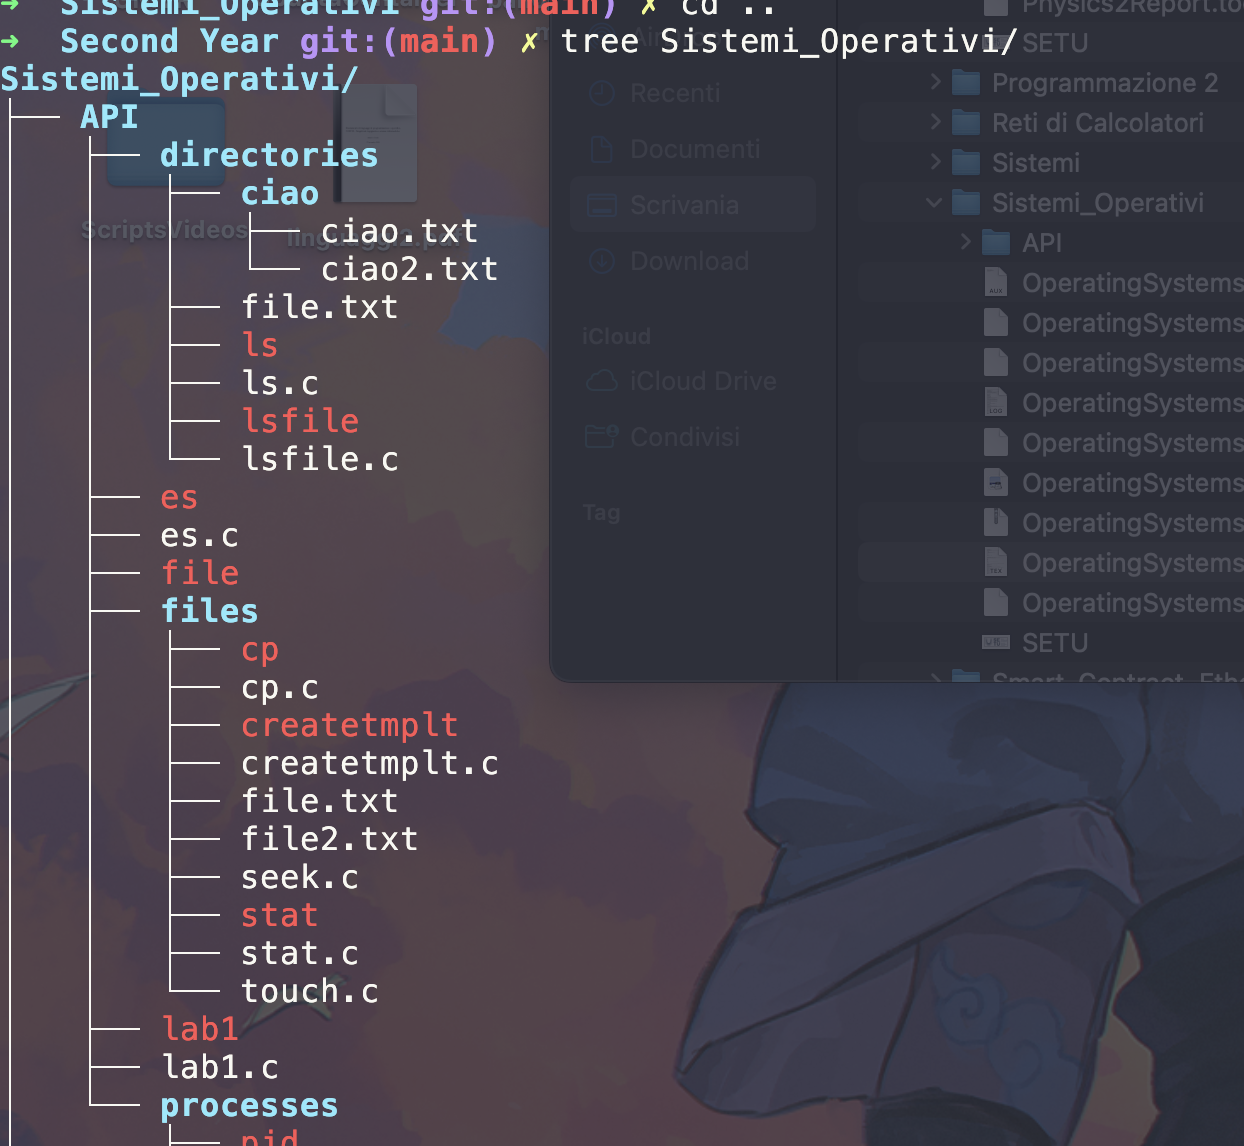
\includegraphics[width=0.6\textwidth]{treeEx.png}
\end{figure}
Displays a simple tree structure of folders in the current directory. To include all files in the display:
\begin{lstlisting}[language=bash]
tree /f
\end{lstlisting}
The /F option lists all files along with the folder structure.
\item Type - The type command is used to display the contents of a text file.   
\begin{lstlisting}[language=bash]
type MyFile.txt
\end{lstlisting}
This displays the contents of the file MyFile.txt. Useful for quickly viewing small text files without opening them.
\item Ver - The ver command is used to display the version of the operating system.
\begin{lstlisting}[language=bash]
ver
\end{lstlisting}
This displays the version of the operating system.


\end{itemize}
\textcolor{green!50!black}{What’s the purpose of the first line - @ECHO OFF? Remove it and see the
effect}

\begin{lstlisting}[language=bash]
@ECHO OFF
ECHO Please insert a USB memory stick
PAUSE
COPY *.txt I:\
ECHO BACKUP COMPLETE
\end{lstlisting}
\begin{itemize}
    \item @ECHO OFF → Hides command execution lines for cleaner output.
    \item ECHO → Displays messages on the screen.
    \item PAUSE → Waits for the user to press a key before continuing.
    \item COPY *.txt I:\ → Copies all .txt files from the current folder to the USB drive (assuming it's drive I:).
    \item ECHO BACKUP COMPLETE → Displays a completion message.
\end{itemize}
The first line, @ECHO OFF, is used to prevent the command prompt from displaying each command as it executes.
\begin{lstlisting}[language=bash]
C:\Users\YourName\Desktop> ECHO Please insert a USB memory stick
Please insert a USB memory stick

C:\Users\YourName\Desktop> PAUSE
Press any key to continue . . .

C:\Users\YourName\Desktop> COPY *.txt I:\
3 file(s) copied.

C:\Users\YourName\Desktop> ECHO BACKUP COMPLETE
BACKUP COMPLETE
\end{lstlisting}

\section{Practical 2 -  Powershell}

\textcolor{green!50!black}{
    2.1 Test the above using a directory that you created last week.
}

\begin{figure}[H]
    \centering
    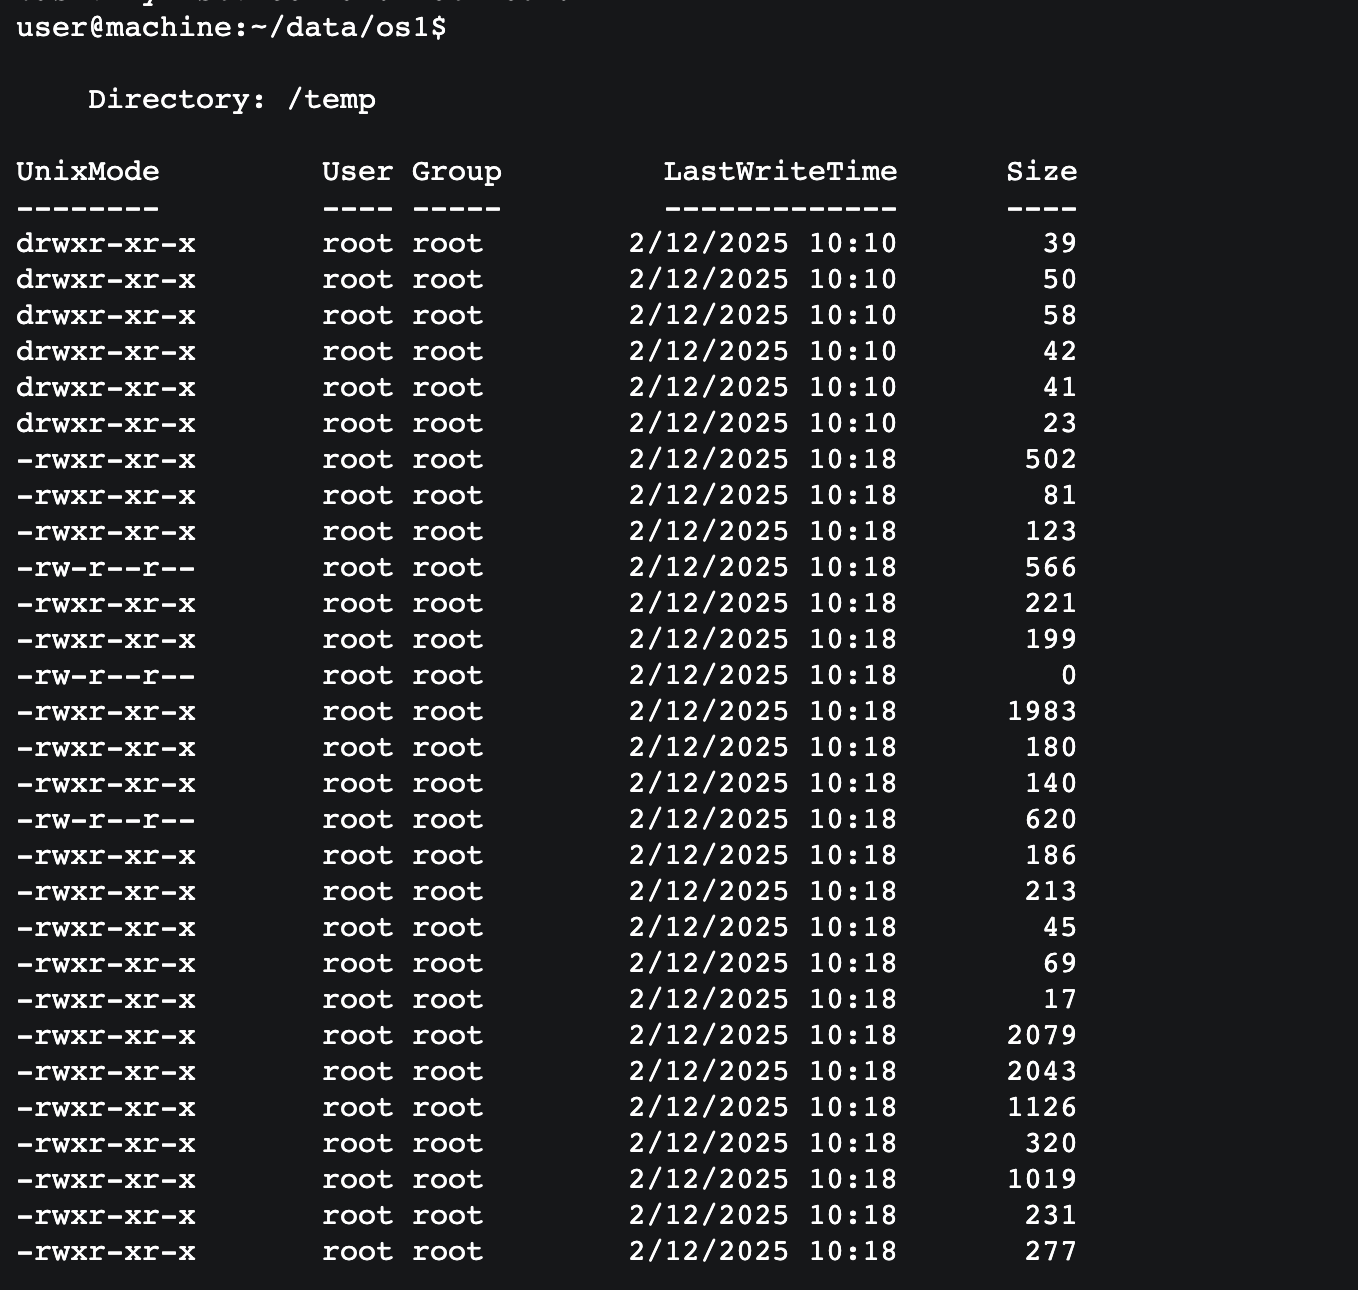
\includegraphics[width=0.6\textwidth]{os1.png}
\end{figure}
\noindent
Using the directory was created last week, we can use the Get-ChildItem command to list the contents of the directory.
using the following list of commands:
\begin{minted}{bash}
$mylist = dir 
$mylist
$mylist[0].Name
$mylist[0].length
$mylist[0].Mode
$mylist[0].LastWriteTime
\end{minted}
\noindent
\textcolor{green!50!black}{
Exercise of bash scripting in Powershell:
\begin{itemize}
    \item Simply record what happens when you run this script.
    \item Find out how to run scripts if they’re in a directory other than the working directory.
    \item Study the following script and see if you can figure out what it’ll do. Now type it into a file called game.ps1 (You can use copy/paste in places to reduce the labour.) Run it and see if your predictions are true.
\end{itemize}
}

\begin{minted}{bash}
###########################################################
###########################################################
##
## The three pathetic knock-knock jokes program!
## Date: 26/09/17
## For: BSc (Hons) Computer Forensics and Security
##
###########################################################
###########################################################

############################
## initialisation section
############################
$userReply = ""
############################
## first question
############################
Clear-Host

while($userReply -ne "Who is there?"){
    $userReply = read-host "Knock Knock!"
}
Clear-Host
while($userReply -ne "Orange who?"){
    $userReply = read-host "Orange"
}
Clear-Host
Write-Output "Orange you glad you created this PowerShell script?"
Start-Sleep -Seconds 5
############################
## Second Question
############################
Clear-Host
while($userReply -ne "Who is there?"){
    $userReply = read-host "Knock Knock!"
}
Clear-Host
while($userReply -ne "Orange who?"){
    $userReply = read-host "Orange"
}
Clear-Host
Write-Output "Oranges are oranges but this is PowerShellscripting!"
Start-Sleep -Seconds 5
############################
## Third Question
############################
Clear-Host
while($userReply -ne "Who is there?"){
    $userReply = read-host "Knock Knock!"
}
Clear-Host
while($userReply -ne "Banana who?"){
    $userReply = read-host "Banana"
}
Clear-Host
Write-Output "Orange you glad I didn't say orange?"
Start-Sleep -Seconds 5
############################
## Farewell Message
############################
Clear-Host
Write-Output "Goodbye!nn"    
\end{minted}
When you run game.ps1, here’s the interactive sequence you’ll experience:

\begin{enumerate}
    \item The script will prompt you with “Knock Knock!”
    \item You’ll need to respond with “Who is there?”
    \item The script will then prompt you with “Orange”
    \item Until you respond with “Orange who?”
    \item The script will then output “Orange you glad you created this PowerShell script?”
    \item The second and third questions follow a similar pattern.
    \item The script will then output “Goodbye!”
\end{enumerate}
\textcolor{green!50!black}{
To do:
\begin{enumerate}
    \item Create another file called beverage.txt identical to drink.txt.
    (Hint: Use what you learned in practical 1 to do this.)
    \item Issue this command again\\
    Get-ChildItem | select-string coffee\\
    and see what happens.
    \item Create a file called fruit.txt with the list apple, orange, banana in it.
    \item Issue this command again\\
    Get-ChildItem | select-string coffee\\
    and see what happens.
\end{enumerate}
}
\begin{minted}{bash}

PS C:\Users\User1\green> Copy-Item drink.txt beverage.txt
PS C:\Users\User1\green> Get-ChildItem *.txt
Directory: C:\Users\User1\green

Mode                LastWriteTime         Length Name
----                -------------         ------ ----
-a----        2/10/2025   10:15 AM           123 drink.txt
-a----        2/10/2025   10:15 AM           123 beverage.txt
PS C:\Users\User1\green> Get-ChildItem | Select-String coffee
drink.txt:1:coffee.
beverage.txt:1:coffee.
PS C:\Users\User1\green> Set-Content fruit.txt -Value "apple`r`norange`r`nbanana"
PS C:\Users\User1\green> Get-Content fruit.txt
apple
orange
banana
PS C:\Users\User1\green> Get-ChildItem | Select-String coffee
drink.txt:1:coffee.
beverage.txt:1:coffee.
\end{minted}
\noindent
\textcolor{green!50!black}{
Find out and explain how to get help about any cmdlet.
\begin{itemize}
    \item Find out and explain what F7 does in PowerShell.
    \item  What is the purposes of (a) the –whatif switch and (b) the –confirm
    \item Write a note to explain how you can use tab to complete a command as soon as
    it’s unambiguous.  
\end{itemize}
}
\noindent
In PowerShell, you can obtain help for any cmdlet by typing Get-Help followed by the name of the cmdlet.
\begin{minted}{bash}
Get-Help Get-Process
\end{minted}
This will display detailed information about the Get-Process cmdlet, including a description, syntax, parameters, examples, and more.
When you press F7 in a PowerShell console, it brings up a graphical popup window displaying your command history from the current session.
You can use the arrow keys to navigate through the list of previously executed commands. This is a handy feature to quickly recall and reuse commands without retyping them.
\\
The -WhatIf switch is used to simulate the execution of a command. It shows you what would happen if the command ran but does not make any actual changes.
Use -WhatIf with potentially destructive or impactful commands to verify what actions would be performed.
\begin{minted}{bash}
Remove-Item C:\Temp\* -WhatIf
\end{minted}
The -Confirm switch forces the command to prompt for your confirmation before executing each action. This extra safety measure helps prevent accidental changes.
\begin{minted}{bash}
Remove-Item C:\Temp\* -Confirm
\end{minted}
\noindent
PowerShell supports intelligent tab completion. As you start typing a command, cmdlet name, parameter, or even file path, you can press the Tab key to auto-complete the text.
If the text you've entered uniquely identifies a command or parameter, pressing Tab will automatically complete it.
If \textbf{multiple completions are possible repeatedly pressing Tab cycles through the available options until you reach the one you want.}








\end{document}